\chapter{基于渐进式策略的多阶段人体运动姿态预测框架}\label{chapter-5}
本章节将围绕本文的一个主要贡献点——基于渐进式策略的多阶段人体运动姿态预测框架进行介绍。分别从动机、方案、实现和算法细节几个方面对本方法进行详细的阐述。在此之前,本文首先通过数学语言定义人体运动姿态预测问题,并介绍在此过程中使用的相关数据结构,以方便在本文后续章节中进行准确的叙述。
\section{人体运动姿态预测问题的数据描述与问题定义}
\subsection{人体运动姿态数据结构}
\begin{figure}[ht]
    \centering
    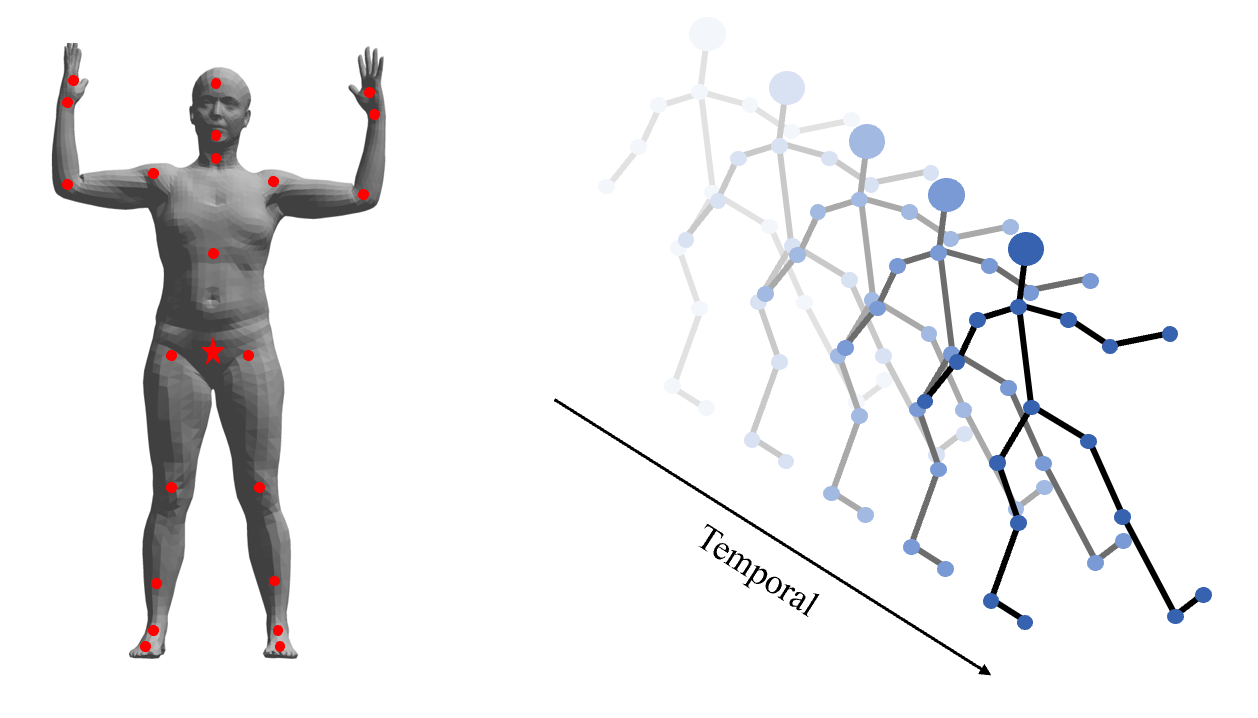
\includegraphics[width=0.85\textwidth]{FigMa/show_structure.png}\\
    \vspace{-0.3cm}
    \caption{人体运动姿态数据结构}
    \label{fig:data_structure}
\end{figure}
首先介绍人体运动姿态预测问题所使用的数据结构。如图\ref{fig:data_structure}左所示,人体运动数据是通过动作捕捉设备,在封闭室内或开放室外场景中提取到的人体关键点运动序列,这些数据以SKT(Skeletal Kinematic Tree)的形式表示和存储。在实际动作捕捉过程中,通常只关注在运动过程中起决定性作用的关节点,例如手肘、肩部、膝盖等。这些关节点在图\ref{fig:data_structure}左中以红色标记的形式展现。其中位于胯部的五角星节点被称为根节点,其余节点的位置通过递归地计算自身对于根节点的相对位置得到。由于本文仅关注三维欧式空间中的人体运动姿态问题,因此,本文用与根节点的相对3D坐标来描述每个关节点空间位置。将通过动作捕捉得到的独立关节点运动序列按照人体空间结构连接后,即可得到抽象后人体运动姿态数据。该数据同时包含时间和空间两个维度的关节点,在图\ref{fig:data_structure}右中,空间维度上描述人体空间结构信息,时间维度上描述关节点序列运动信息。

\subsection{人体运动姿态预测问题定义}
从数学上,对于一个长度为$T$的人体运动序列,本文将其定义为$S_{1:T} = \{P_1,P_2,\cdots,P_{T}\}$,其中$P_i$为运动序列中位于$i$时刻的人体姿态。每个人体姿态$P_i$又由若干个关节点组成,其中$P \in \mathbb{R}^V$,$V$为该人体姿态包含的关节点数量,每个关节点又由一个$D$维的向量描述。

对于人体运动姿态预测问题,网络$\Phi$接收已知输入序列$S_{1:T_h} = \{P_1,P_2,\cdots,P_{T_h}\}$作为输入,预测未来运动序列$S_{T_h+1:T_h+T_f} = \{P_{T_h+1},P_{T_h+2},\cdots,P_{T_h+T_f}\}$,这一过程的数学描述如公式\ref{equation:problem_formulation}所示。其中$\theta$为可训练的网络参数。
\begin{equation}
    S_{T_h+1:T_h+T_f} = \Phi(S_{1:T_h}, \theta) \label{equation:problem_formulation}
\end{equation}

\section{从单阶段网络进化到渐进式多阶段网络}
%\subsection{网络输入输出差异对预测的影响}
\subsection{对单阶段网络中预测不确定性的分析}
正如\ref{section:1.1}节所提到的,预测过程中的不确定性是影响预测精确度进一步提升的关键因素,而这种不确定性来自输入运动序列和待预测序列之间的差异。简而言之,由于输入运动序列和待预测运动序列之间存在较大差异(例如,输入运动和待预测运动属于不同的运动模式),网络无法根据输入序列中的信息来准确推测未来运动,导致预测结果脱离真值。因此,如何降低预测过程中的不确定性成为了提升网络预测精确性的一个重要问题。

在调研过程中,本文注意到LTD\parencite{mao2019learning}提出的一项改进措施使得预测精度相较于现有方法得到了大幅提升。在早期的方法中,如公式\ref{equation:problem_formulation}所示,输入运动序列长度$1:T_h$与待预测序列长度$T_h+1:T_h+T_f$通常存在差异,待预测序列的长度要远远长于输入序列(例如,输入10帧预测25帧),这使得网络需要在输入输出数据存在维度差异的情况下进行预测。这会导致已知和预测序列间的过渡部分不连续,产生较大的预测误差。针对该现象,LTD\parencite{mao2019learning}提出公式\ref{equation:padding},使用输入序列的最后一帧来填充输入序列,使得输入序列和待预测序列保持维度一致。
\begin{equation}
    \begin{aligned}
        &\widetilde{S}_{1:T_h} = [S_{1:T_h}, \{P^{T_h+1}_{T_h}, \cdots, P^{T_f}_{T_h} \} ]
        \\
        &S_{T_h+1:T_h+T_f} = \Phi(\widetilde{S}_{1:T_h}, \theta)
    \end{aligned}
    \label{equation:padding}
\end{equation}

从图\ref{fig:LTD_padding}可以看到,经过填充后的输入数据对网络有两点积极作用。第一,输入和输出维度一致,避免了数据维度差异所带来的不确定性。第二,网络在预测未来运动序列时可以在已知部分最后一帧基础上进行预测,降低了预测的难度。
\begin{figure}[ht]
    \centering
    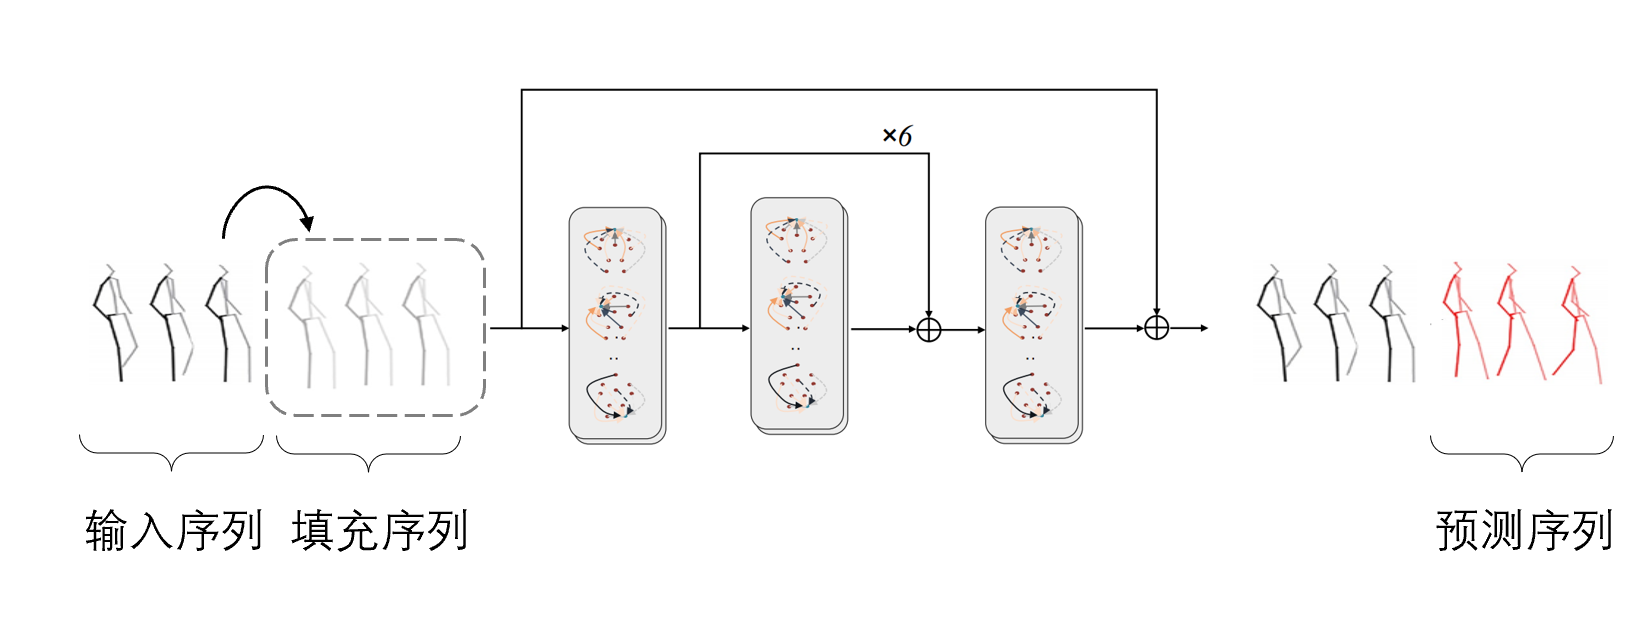
\includegraphics[width=1\textwidth]{FigMa/LTD_padding.png}\\
    \vspace{-0.3cm}
    \caption{LTD数据填充过程}
    \label{fig:LTD_padding}
\end{figure}
然而这种粗糙的填补方法也有其固有缺陷。整个填充过程不考虑不同时序位置在预测难度上的差异,全部使用最后一帧进行填充,对于离$P_{T_h}$较近的未来运动,$P_{T_h}$还能提供一定的参考。随着时间向前,未来帧与$P_{T_h}$的关联越来越弱,其提供的参考价值也越来越低,预测的不确定性也逐渐增加。因此该填充方法无法缓解较远距离的预测不确定问题。

LTD证明了通过消除输入数据和预测目标之间的维度差异,可以有效降低预测不确定性。而本文希望验证,缩小二者在内容上的差异也能达到同样的效果。因此,本文以LTD为基准模型,设计了图\ref{fig:toy_experiment}中所示的验证实验。在实验中,预测目标保持不变,输入数据的填充内容被替换为部分预测目标的均值。例如图\ref{fig:toy_experiment}中所示,使用真值中前$L$帧的均值进行填充。直觉上,填入均值相当于向输入数据泄露了部分预测目标的信息,直接缩短了二者在内容上的差距,进而大幅降低了预测难度。图\ref{fig:toy_experiment}展示的结果也验证了本文的猜想,以均值形式混入的预测目标信息显著缩短了输入数据和预测目标之间的差距,整体预测精度相较于LTD有了明显提升,且混入的信息越多对应位置以及整体上预测精度提升幅度越大。

\begin{figure}[h]
    \centering
    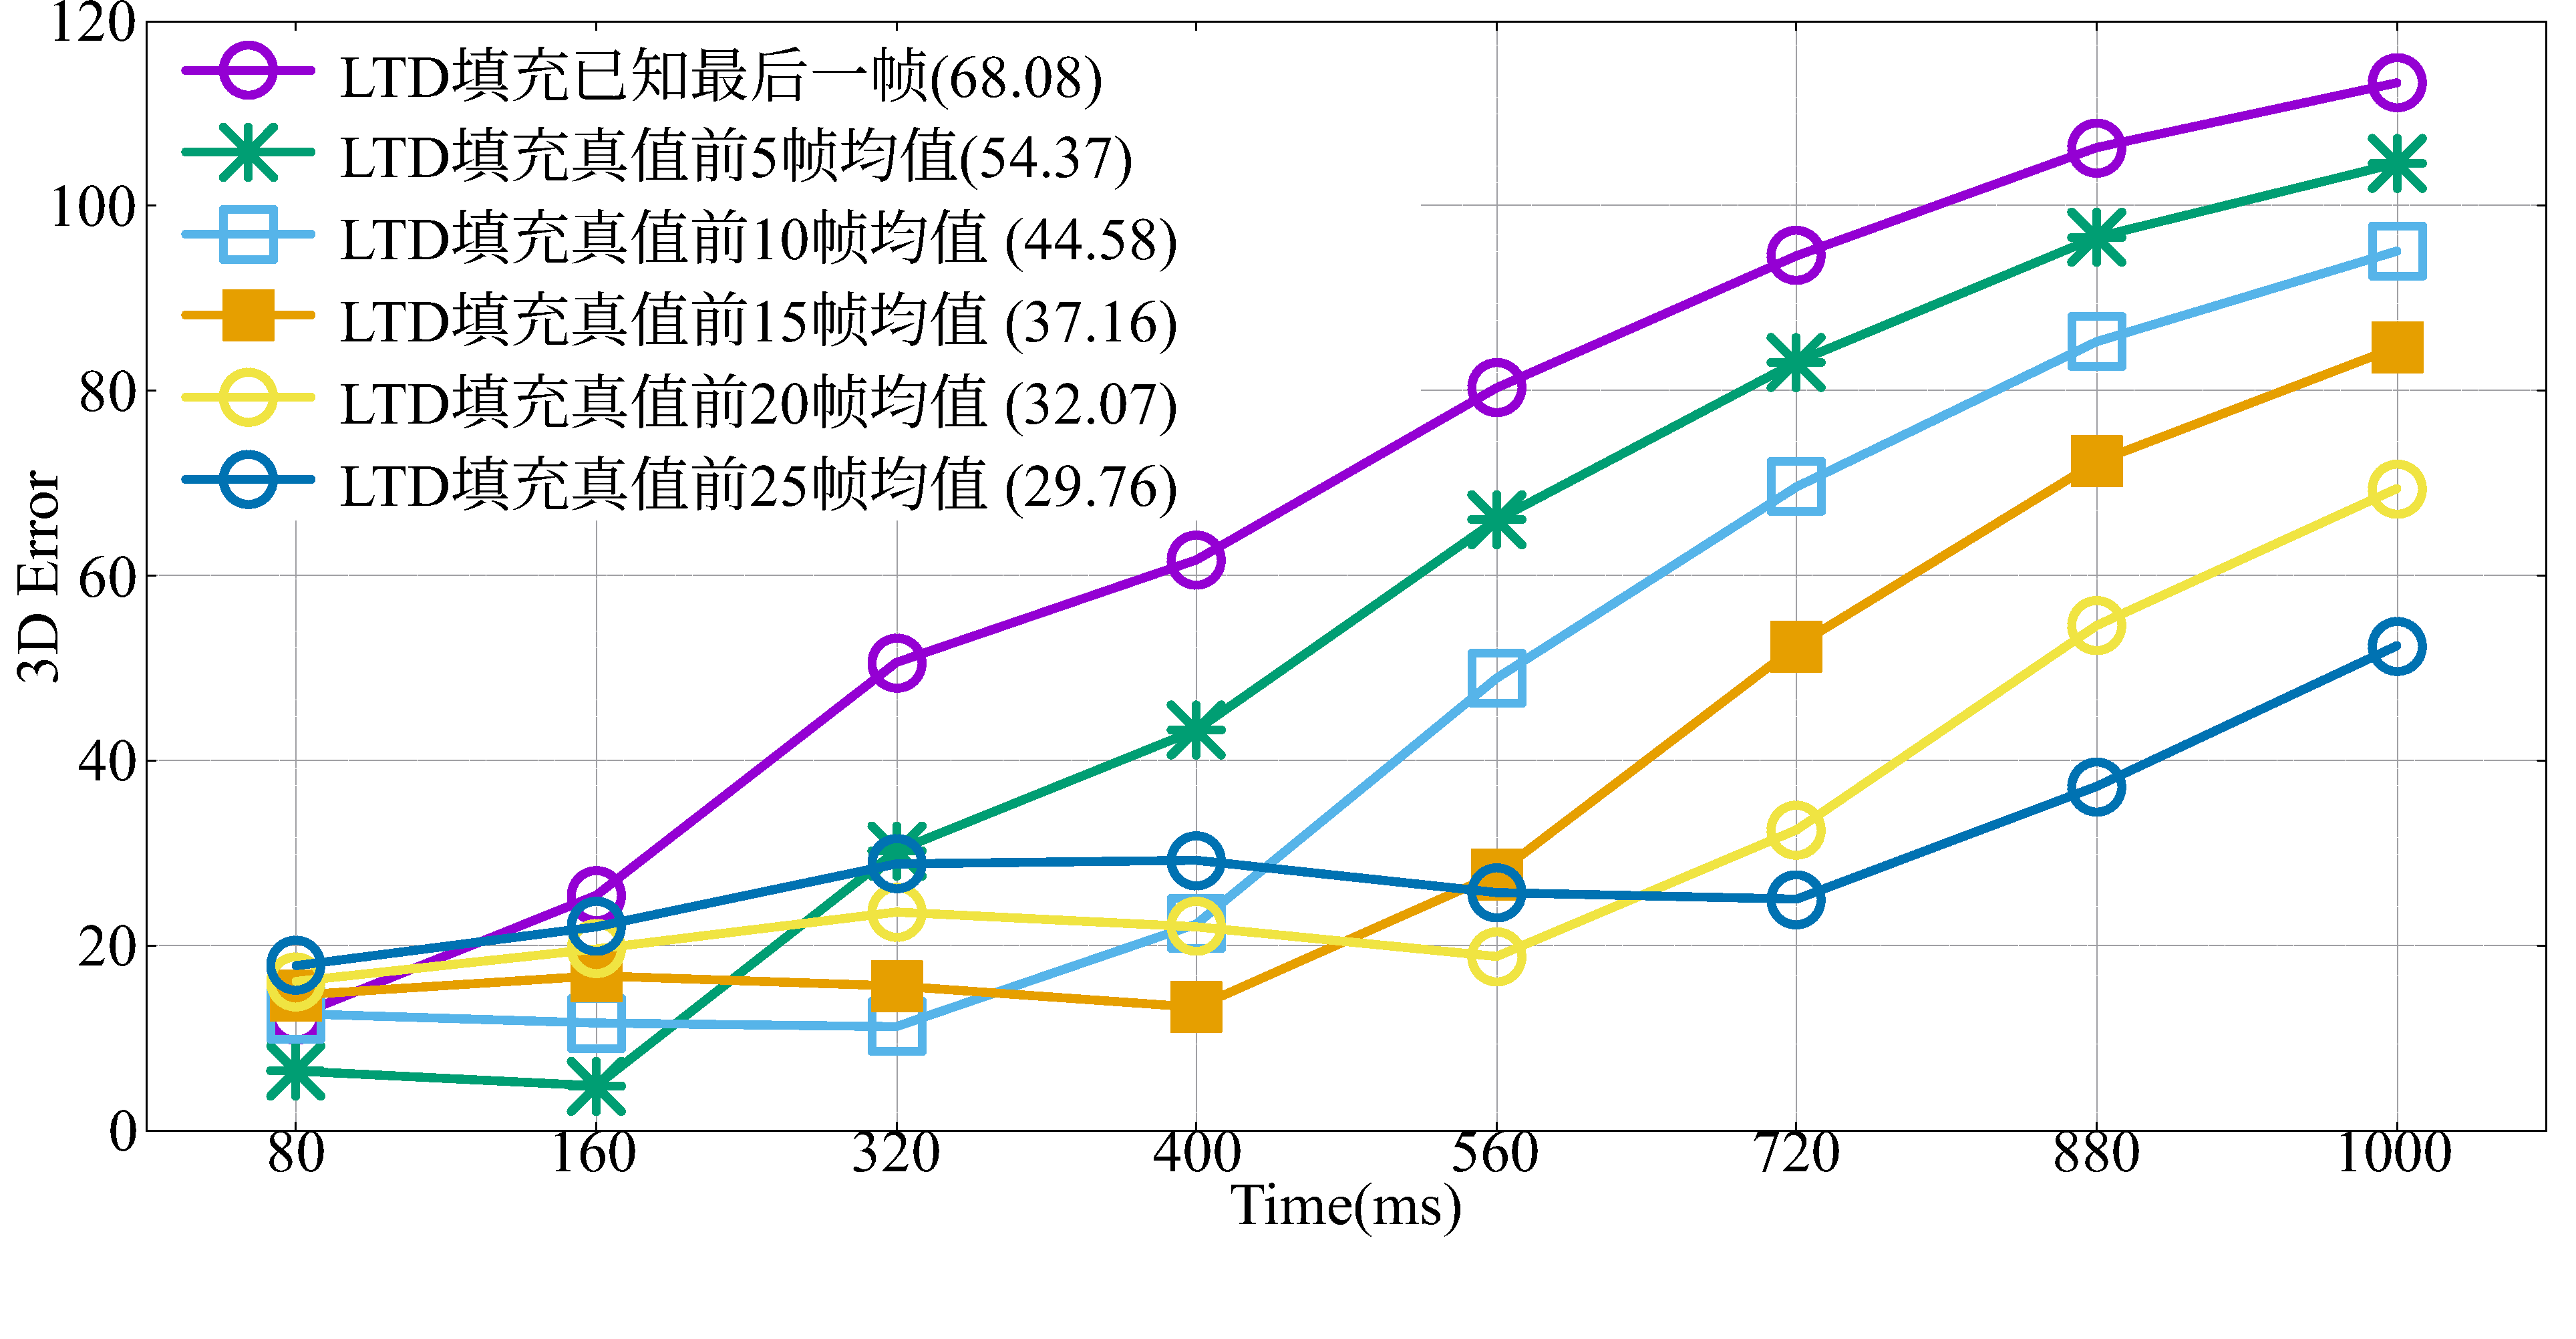
\includegraphics[width=0.8\textwidth]{FigMa/padding_chinese.pdf}\\
    \vspace{-0.3cm}
    \caption{基于LTD的不同内容填充实验}
    \label{fig:toy_experiment}
\end{figure}

\subsection{通过Coarse to fine二阶段网络降低预测不确定性}
在分析上述结果后,本文认为,缩小输入序列和待预测序列的差异(维度差异、内容差异等)可以有效降低预测过程中的不确定性,大幅提高预测的精确性。但将最后一帧作为输入序列的填充,显然并非一个好的选择。

由于在实际预测场景中,无法将预测目标信息泄露给输入数据,因此无法参考图\ref{fig:toy_experiment}中的做法,直接使用真值均值填充输入序列。受到最近被广泛应用的由粗糙到精细(Coarse to fine)策略的启发,本文希望通过分割预测任务,将预测模型分为两个阶段,两个阶段各负责一部分预测任务的方式降低整体的预测不确定性。具体地,Coarse to fine 策略与大多数单阶段预测的方法不同,预测被分为了两个阶段。位于网络浅层的阶段被称为粗糙(Coarse)网络,它接收原始的输入,并输出一个较为粗糙的结果,虽然该结果离最终的目标存在一定的偏差,但与最初的输入信息相比,它已经包含了真值中的绝大部分运动趋势。随后该粗糙结果被送入精修(Fine)网络,精修网络将在粗糙网络的基础上进一步完善运动细节。该策略被广泛应用于图片修复(Image Inpainting)\parencite{yu2018generative,zamir2021multi}领域,在该类方法中,原始缺失图片通常由粗糙网络生成一个低分辨率较模糊的修复版本,此次修复的目的是修复图片内容的结构。随后,粗修版本被送入精修网络提高分辨率并进一步完善细节,最后输出高质量的修复结果。参考该思路,本文设计了一个Coarse to fine 人体运动姿态预测网络。

\begin{figure}[ht]
    \centering
    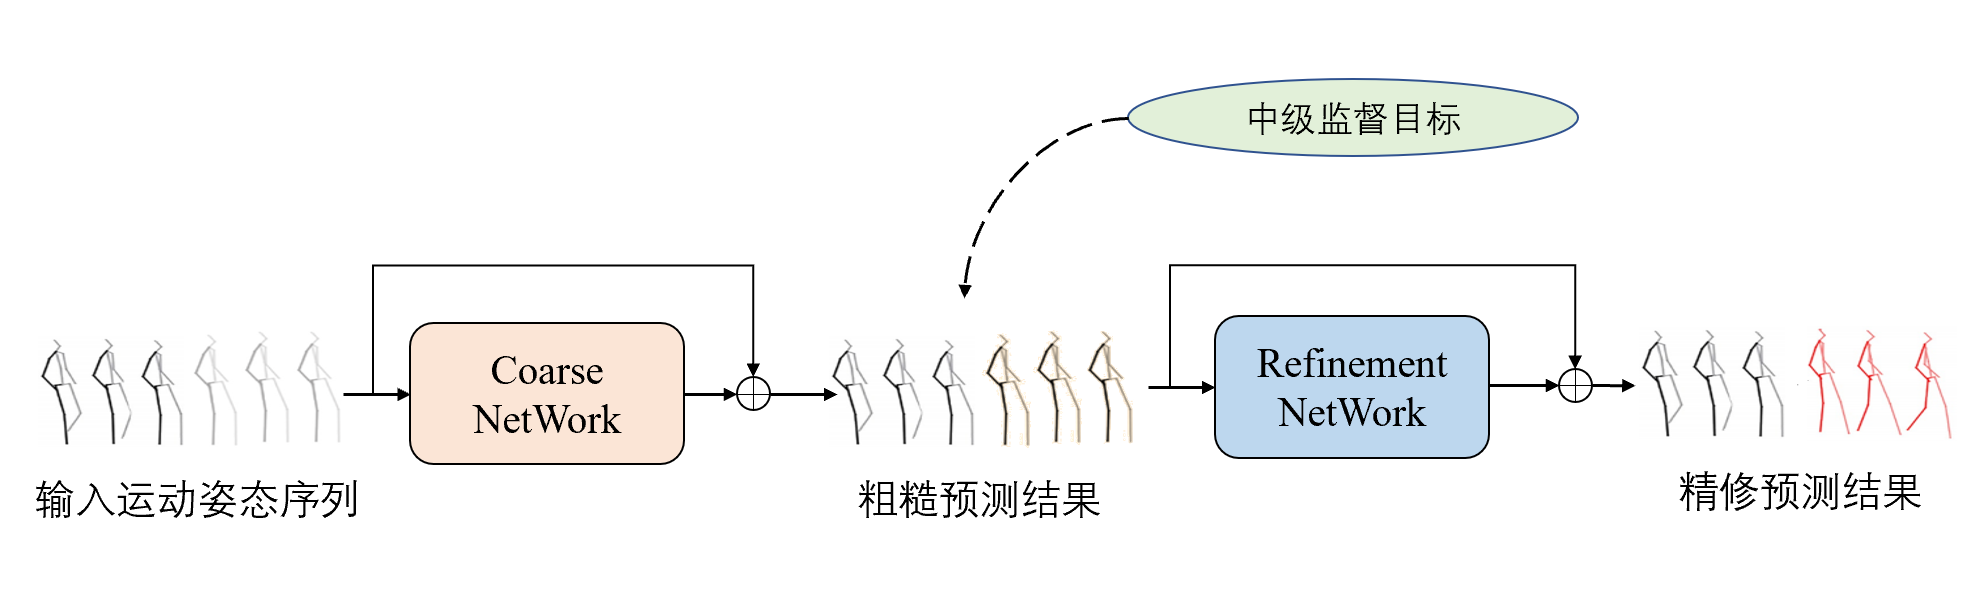
\includegraphics[width=0.8\textwidth]{FigMa/Two_stage.png}\\
    \vspace{-0.3cm}
    \caption{Coarse to fine 二阶段预测网络}
    \label{fig:Two_stage}
\end{figure}

在最初的粗修阶段中,本文仍然保留了LTD中基于最后一帧的填充步骤,因为此步骤可以保证网络输入输出维度一致,减少维度上的不确定性。经过填充后的输入序列经过粗修网络,预测得到一个较为粗糙的结果,该结果受到中级监督目标的监督。该中级监督目标相比较最终的预测目标,去除了部分运动细节,只保留了运动大致趋势。随后,粗糙的预测结果被送入后续的精修网络,进一步丰富动作的细节。此时,预测结果受到最终预测目标的监督,以期望获得与真值一致的结果。该模型通过两阶段的结构,将预测过程拆分为两个部分,显著缩小了输入数据和预测目标间的内容差异,大大降低了预测的不确定性。最终,预测精确性与单阶段的LTD网络相比有显著提升(3D预测误差对比:LTD(68.3),Coarse to fine二阶段预测网络(66.9))。
%\subsection{渐进式多阶段预测网络框架}
\subsection{从二阶段网络推广到渐进式多阶段网络}
随后本文进一步拓展了该网络,将一个两阶段的Coarse to fine网络拓展为多阶段的网络。通过对预测过程的进一步细分,每个阶段的预测难度被进一步降低,网络也容易做出准确的预测。本文将多阶段的网络模型定义如下。
\begin{equation}
    \begin{aligned}
         \hat{S}_{1:L}^{1} &= \Phi^1([{S}_{1:T_h};P_{T_h},\cdots,P_{T_h}]), \\
        \hat{S}_{1:L}^{i} &= \Phi^i([S_{1:T_h};\hat{S}_{T_h+1:L}^{i-1}]), i = {2,3,\cdots,T},
    \end{aligned}
    \label{equation:multi-stage_formulation}
\end{equation}
公式\ref{equation:multi-stage_formulation}中,现有方法中单阶段的预测过程$\Phi$被拆分为多个阶段$\Phi = \{ \Phi_1, \cdots, \Phi_T\}$,每个阶段在上一个阶段的预测基础上,不断完善运动细节,使得预测精确度不断稳步提升。相比较现有的单阶段网络,多阶段网络预测过程更加可控,每阶段的预测结构都受到与之对应的中级监督目标的监督,此外预测任务的细分也使得每阶段网络的预测不确定性进一步降低,预测难度也进一步降低。最终,本文设计了一个多阶段的网络,其网络结构图如图\ref{fig:multi_stage}所示。

多阶段的网络设计包含两点,第一是每个阶段(Stage)的子网络设计,在这里暂时使用了LTD中提出的GCN模块(在文章后续内容中本文提出了具有更强时空信息提取能力的ST-DGCN模块用以替换)。每个子网络内部为一个前馈神经网络网络(Feed forward network)。内部由$n$个GCB(GCN Block)构成,每个GCB又由两个GCL(GCN Layer)构成,GCL是网络的最基本的构成结构,其具体结构如图\ref{fig:multi_stage}右下角所示,GCL由一个GCN、BatchNorm、Tanh和DropOut组成,可以完成最基本的人体运动姿态时空信息提取功能。值得注意的是,网络的规模并不随着阶段数量的增加而提升,在本文的设计中,网络中的GCB数量固定,随着阶段的增加,每个阶段包含的GCB数量等比例下降。
\begin{figure}[ht]
    \centering
    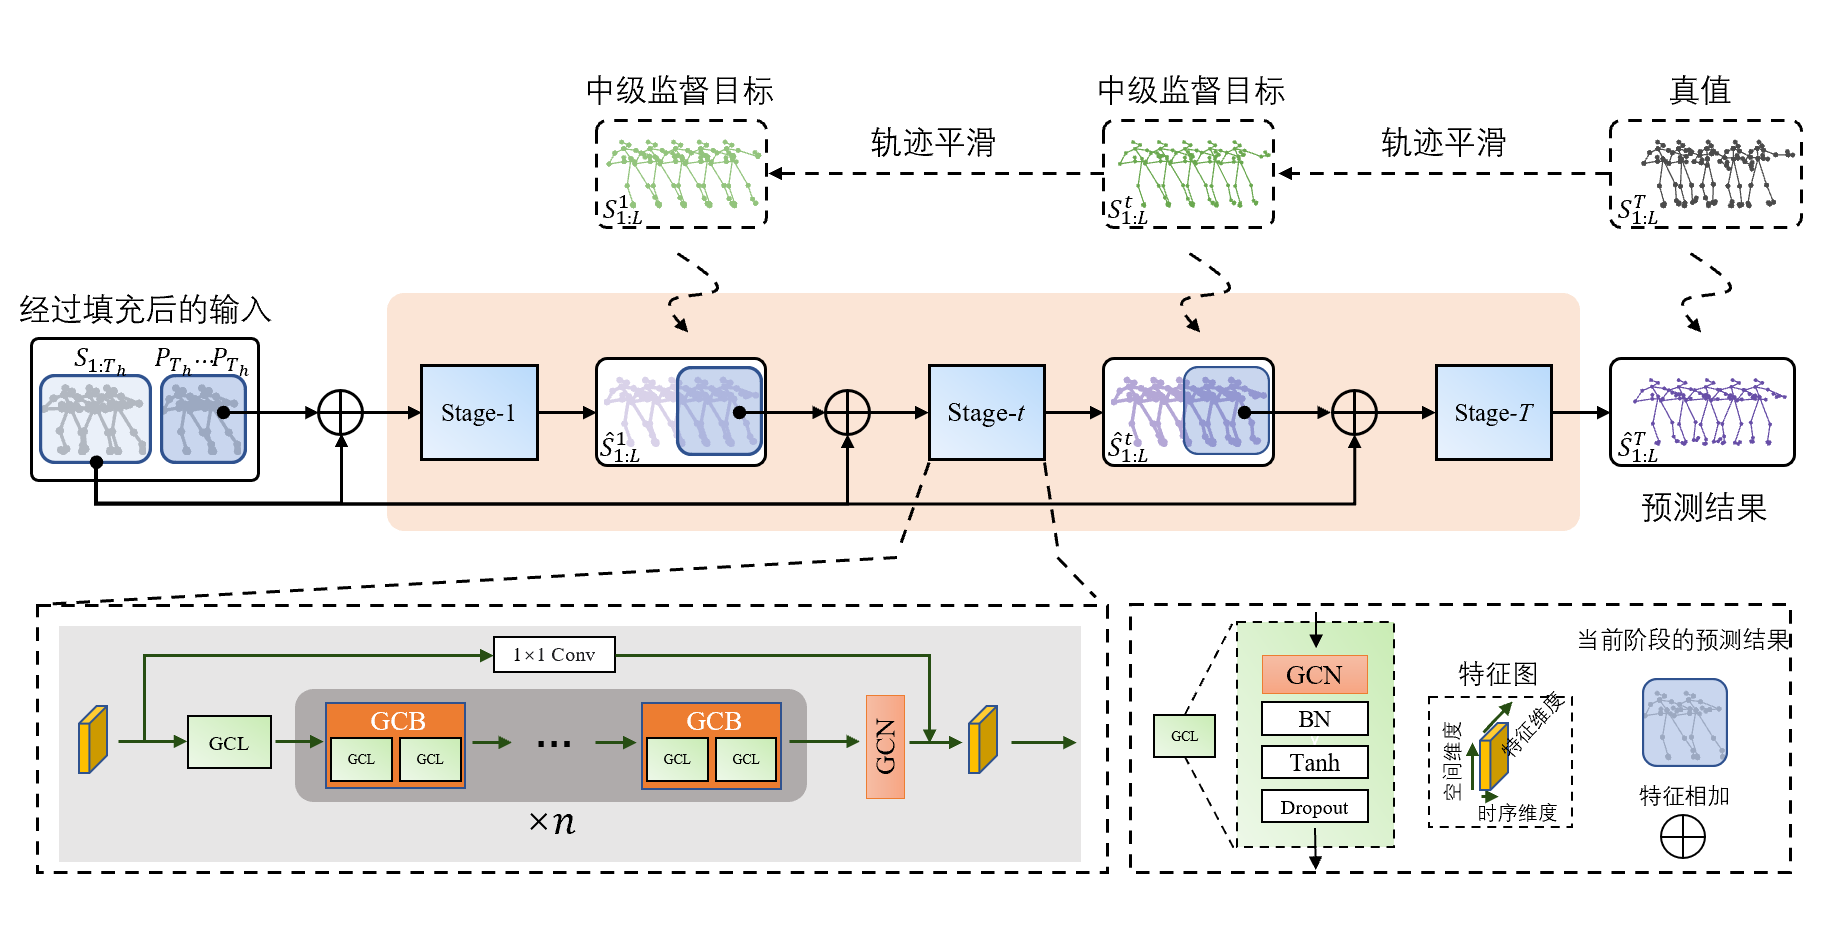
\includegraphics[width=1\textwidth]{FigMa/multi-stage_network.png}\\
    \vspace{-0.3cm}
    \caption{渐进式多阶段的预测网络}
    \label{fig:multi_stage}
\end{figure}
网络参数量的增加在一定程度上提高了网络的容量和表达能力,但当突破某一阈值的时候网络复杂度增加带来的计算开销负担抵消了这一优势。所以,本文的多阶段网络,通过控制网络中的GCB数量,在提升网络性能的同时,维持了网络规模基本不变。

第二点是中级监督目标的设计,中级监督目标必须具有层次化特点,遵循由简单到复杂的原则,浅层网络负责较为简单的整体运动趋势预测,而深层网络负责较为复杂的细节完善任务。在其他类型任务(图像等规则数据)的中级监督目标设计中,可以简单地通过降低分辨率、模糊处理和提取边缘特征等方式降低图片的细节或提取内容的结构信息来构造中级监督目标。但人体运动姿态数据是不规则的拓扑数据。无法通过常规的降维手段提取结构信息或降低运动复杂度。虽然当前也有一些方法,如MSR\parencite{dang2021msr}提出在空间维度上对人体结构进行降维,合并运动模型类似的相邻关节点来减少图中的关节点数量,构造具有空间层次结构的中级监督目标。但该方法破坏了重要的人体结构先验信息,抵消了渐进式多阶段策略对网络性能的提升。

\subsection{渐进式多阶段网络中的中级监督目标构造方法}
本文设计了一种适用于人体运动姿态数据的中级监督目标构建方法,该方法可以在保持原有的空间结构的同时,降低时间维度上的关节点运动复杂度。具体地,本文在不同阶段对关节点轨迹施加不同强度的平滑算法作为中级监督目标。网络浅层因为表达能力不足,因此其对应的中级监督目标被施加了更强的平滑来降低运动的复杂度和预测难度。随着网络深入,网络的表达能力增加,能够承担更复杂的预测任务。此时,对于中级监督目标的平滑程度就会被削弱,以帮助其在之前阶段的预测基础上,丰富运动细节。为此,本文设计了一种名为累积均值平滑(Accumulated Average Smoothing,AAS)的方法构造用于人体运动姿态序列预测问题的中级监督目标。

在介绍累积均值平滑算法之前,为了方便叙述,本文首先给出人体运动姿态模型中关节点轨迹的数学定义。假设每个人体姿态包含$V$个关节点,每个关节点由$D$维的向量描述。一个人体运动姿态序列$S_{1:L}$包含$V \times D$条轨迹:$\{T_j|j\in[1, V\times D]\}$,每条轨迹$T_j$由同一个关节点的某位维度上的运动组成:$T_j=\{x^i_j|i\in[1,L]\}$。由于所有轨迹都由同样的平滑方法处理,在下面的叙述中本文忽略了不同轨迹的区别,统一用$T$代称$T_j$。

$T$由两部分组成:已知的运动序列$\{x^i|i\in[1,T_h]\}$和待预测的运动序列$\{x^i|i\in[T_h+1,T_h+T_f]\}$。由于已知的运动序列属于模型的输入数据,不需要预测,所以无需经过平滑算法处理。待预测的真实运动序列则需要用平滑算法调节该部分数据的预测难度。目前被广泛使用的平滑算法是基于高斯卷积核的滤波器。高斯滤波器被广泛应用于图像平滑领域,它是一种常见的线性滤波器。它的原理是将一个二维高斯分布函数应用于图像的每一个像素,使得该像素周围的像素加权平均起来,从而达到平滑图像的目的。高斯滤波器的核心是高斯核(Gaussian kernel),也称为卷积核(Convolution Kernel)或滤波器(Filter)。高斯核是一个二维高斯分布函数,它的中心是图像上的当前像素点。高斯核中的每个元素表示该位置的权重,越靠近中心位置的像素权重越高,越远离中心位置的像素权重越低。通常情况下,高斯核是一个奇数×奇数的矩阵,这样可以保证中心像素的位置。在轨迹平滑算法中,2D的高斯卷积核退化为1D,其卷积核权重计算公式为:
\begin{equation}
    G(x) = \frac{1}{\sqrt{2\pi}\sigma}e^{-\frac{x^2}{2\sigma^2}}
    \label{equation:gauss_filter}
\end{equation}
其中$x$表示当前位置相对于卷积核中心的距离,$\sigma$表示标准差,标准差越大越靠近卷积核中心的权重越高,反之权重分布越平均。
\begin{equation}
    G = \frac{1}{\sqrt{2\pi}\sigma}
        \begin{bmatrix}e^{-\frac{-{((N-1)/2)} ^2}{2\sigma^2}} & \cdots & e^{-\frac{-{((N-1)/2)}^2}{2\sigma^2}} \\ 
        \vdots & \ddots & \vdots \\
        e^{-\frac{0^2}{2\sigma^2}} & \cdots & e^{-\frac{0^2}{2\sigma^2}} \\
        \vdots & \ddots & \vdots \\
        e^{-\frac{{((N-1)/2)}^2}{2\sigma^2}} & \cdots & e^{-\frac{{((N-1)/2)}^2}{2\sigma^2}
        }\end{bmatrix}
    \label{equation:gauss_filter_mat}
\end{equation}
如果需要生成一个$N\times 1$的高斯卷积核,可以通过上述公式\ref{equation:gauss_filter}得到卷积核矩阵\ref{equation:gauss_filter_mat},其中,$G$ 是 $N\times 1$ 的高斯卷积核矩阵,$N$ 表示卷积核的大小。

由于在本问题中,只需要对一条轨迹待预测部分进行平滑,已知的运动序列保持不变即可。而高斯滤波器在对轨迹进行处理时,不可避免地计算卷积核范围内的所有数据,因此在已知运动序列和待预测部分的过渡部分会出现跳跃(Jump)现象,这是由于高斯滤波器在计算过渡部分的平滑值时,将卷积核范围内已知运动序列纳入计算。而已知运动序列在最终的结果中并没有被平滑,所以导致计算结果在该处出现了跳跃现象。此外,由于高斯滤波器在计算时,其节点原始值的权重较高,导致平滑力度不足,难以构造层次化的中级监督目标。

因此,本文提出了累积均值平滑算法来解决以上两个问题。本文将该算法定义如下:

\begin{equation}
    \bar{x}^i = \frac{1}{i-T_h}\sum_{k=T_h+1}^{i}x^k, \forall i\in[T_h+1, T_h+T_f].
    \label{equation:AAS}
\end{equation}

待预测部分的某个节点的平滑值由其之前所有节点的累计平均值得到。首先平滑值计算过程只涉及待预测部分,不涉及已知部分,这就避免了过渡部分的跳跃问题。其次,该节点的平滑值是由前面所有节点的平均值而非加权平均得到的。这意味着每个节点在平滑过程中都具有相等的权重,没有任何一个节点能够主导结果。这种方法消除了原始节点权重过高,影响平滑效果的问题。另外,随着当前节点离已知部分的距离增加,该参与平滑计算的节点数量也逐渐增加,平滑力度也随之增强。这种现象符合一般直觉,距离已知部分较远的节点预测难度更大,需要更强的平滑力度来降低预测难度。相反,靠近已知部分的节点保留了更多的原始信息,这是因为这些节点的不确定性较低,预测难度也相对较低,因此不需要进行过度平滑。因此,该算法能够基于每个节点的不确定性程度和预测难度来自适应地平衡平滑力度和原始信息保留程度。这使得该算法可以在处理各种复杂的预测问题时,提供具有层次化,且更合理的中级监督目标。总之,累积均值平滑算法相比传统的高斯滤波算法能够生成过渡更平滑,难度梯度更合理的中级监督目标,能有效地帮助网络建立一个渐进式的学习框架,降低预测难度,提高网络学习效率。

\begin{figure}[ht]
    \centering
    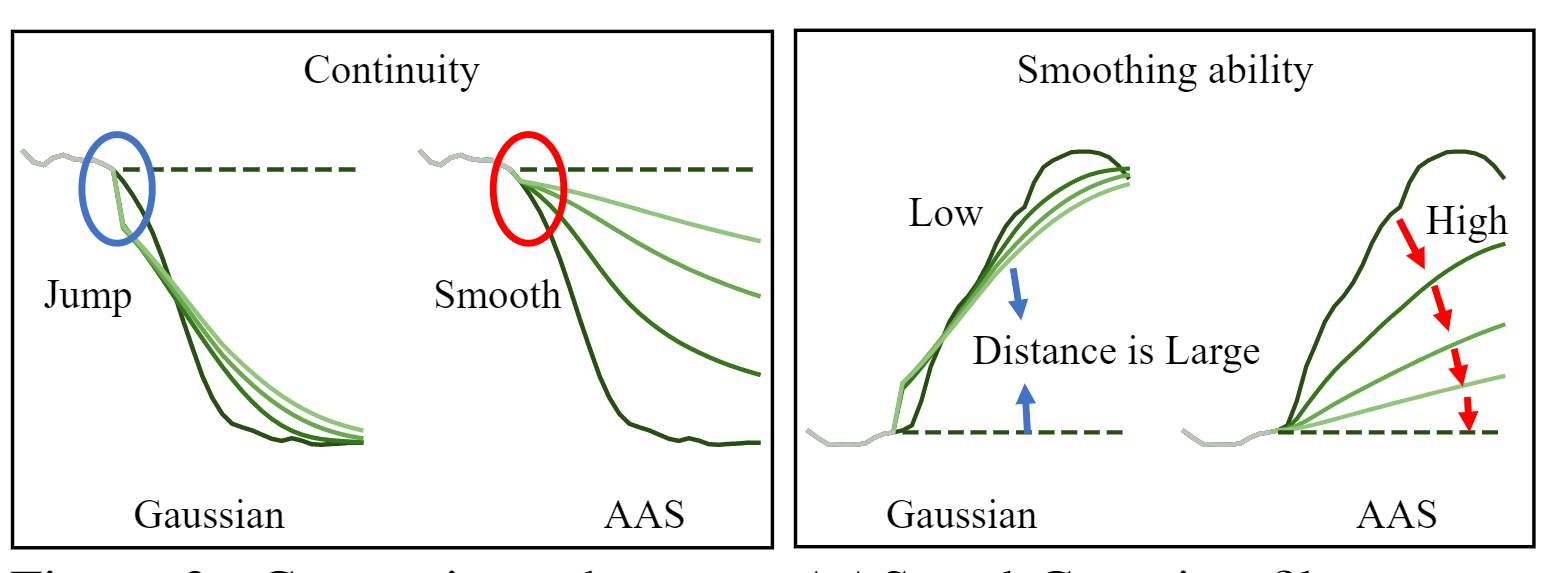
\includegraphics[width=1\textwidth]{FigMa/AAS.png}\\
    \vspace{-0.3cm}
    \caption{累积均值平滑对比高斯滤波}
    \label{fig:AAS}
\end{figure}
图\ref{fig:AAS}展示了累积均值平滑算法(AAS)和高斯滤波算法(Gaussian)的平滑结果对比。其中灰色实线是输入模型的已知运动序列,深绿色虚线是使用已知运动序列最后一帧构成的填充序列。接下来由深到浅的绿色实线是不同阶段的平滑结果。拥有最深颜色的曲线是待预测的真实运动序列,稍浅一点的为经过一次平滑的结果,后续逐渐变浅的线段是经过多次平滑的结果,颜色越浅则经历的平滑次数越多。

图\ref{fig:AAS}左展示了高斯滤波出现的过渡部分跳跃问题。从图中可以看到,待预测的真实轨迹与已知序列的过渡部分是平滑的。然而在经过高斯滤波处理后,平滑后的待预测轨迹与已知部分的连接处,出现了明显的跳跃现象,这是由于在计算该部分平滑值时,卷积核窗口包含了已知序列和待预测序列两部分的信息。而本文提出的累积均值平滑算法解决了这一问题,在对某个节点进行平滑处理时,纳入计算的运动数据只涉及当前节点之前的待预测运动序列,不包含已知运动序列,且平滑的强度随时间增加而线性增长。例如,当计算待预测序列的第一个节点的平滑值时,由于该节点已经位于待预测序列的开始位置,因此,计算该节点的平滑值只需将该节点代入公式\ref{equation:AAS},得到的平滑结果也既是它本身。由于平滑节点数据未发生突变,因此可以和已知部分平滑过渡。

图\ref{fig:AAS}右,展示了累积均值平滑算法和高斯滤波算法的平滑力度对比。在高斯滤波算法的计算过程中,卷积核窗口给予了当前节点过高的权重,导致平滑结果与当前节点的差异较小。最终,即使在经过迭代后的多次平滑步骤。结果的平滑程度仍然较低,无法满足构造层次化的中级监督目标的要求。而在累积均值平滑算法中,采用了累积的策略,越远离已知部分的节点受到的平滑力度越大,其次,使用平均而不是加权平均的算法,平滑结果受到当前节点的影响更小,平滑的结果也更加明显。累积均值平滑算法的平滑结果表明,该算法能够在去除运动细节的同时,保留数据序列的趋势特征。与其他常见的平滑算法相比,累积均值平滑算法在平滑强度方面表现更加优秀。这种层次化的特点使得累积均值平滑算法的平滑结果更加符合渐进式策略中预测目标由易到难的变化趋势,为多阶段预测网络模型提供了更好的中间监督目标。该中间监督目标可以有效地降低预测难度,并提高预测的准确性和稳定性。因此,基于累积均值平滑算法的平滑结果是一种有价值的中间监督目标,它可以帮助多阶段预测网络模型实现更加准确、稳定和可靠的预测结果。

\subsection{总结}
本章介绍了基于渐进式策略的多阶段人体运动姿态预测网络,以及对应渐进式多阶段网络结构的中级监督目标构造方法。首先本文从对现有方法的分析入手,发现现阶段人体运动姿态预测问题的难点在于输入数据和待预测数据之间的差异过大,导致网络预测过程存在不确定性。LTD提出使用已知部分来填充空白维度,使得输出数据达成维度上的统一,消除由于维度差异带来的不确定性。受此启发,本文希望更进一步,通过降低二者在内容上的差异性来消除预测不确定性。为此本文首先设计了一个Coarse to fine二阶段实验网络,人体运动姿态预测被分为两个部分,第一个阶段网络的预测目标是较简单的大致的运动趋势,第二阶段的网络在上一步的基础上完善复杂的运动细节,使最终的网络输出与真值一致。在两阶段的网络中,本文在不增加网络参数量的前提下,通过分解任务的方式将缩小了各个阶段中,输入与输出之间内容上的差距,从而降低了预测的不确定性。在最终的设计中,本文将两阶段的网络推广到多阶段的网络,进一步体现渐进式策略的优势。

本文的另一个贡献点是提出了一种名为累积均值平滑的中级监督目标构造方法,该方法相比较常用的高斯滤波平滑方法,可以避免平滑后运动序列的过渡部分出现跳跃现象。此外,由于其累积平滑的特性,拥有更强的平滑能力,相比高斯滤波平滑能够生成更具层次化的中级监督目标,辅助多阶段网络构建一个从难到易的网络预测框架。

除了通过基于渐进式策略的多阶段网络结构来降低输入数据和预测目标内容上的差距,本文还期望提高网络中的基础图卷积模块的时空信息提取能力,来降低预测过程的不确定性。现有图卷积模块或缺失了对时序信息的建模,或感受野范围受限于传统算子的卷积核大小,又或是带来了不可接受的网络规模膨胀。而本文希望提出一种在不显著提升时空开销的前提下,拥有对时空信息高效建模能力的GCN模块。本文将在下一节详细阐述该方案。